\chapter{Data}


\section{CAP Sleep Database}

The EEG dataset used in this study was obtained from PhysioNet’s publicly available CAP Sleep Database \parencite{goldberger2000physiobank}. The sleep scoring was conducted by a team of experts from the Sleep Disorders Centre at Ospedale Maggiore in Parma, Italy.. \\

The CAP Sleep Database comprises 108 PSG recordings, all collected at the same medical center. These recordings include multiple physiological signals, such as at least three EEG channels C3 or C4, F3 or F4, and O1 or O2 referenced to A1 or A2. Additionally, the dataset contains EOG channels, submental muscle EMG, respiration signals, bilateral tibial EMG, and one EKG. The EEG recordings also include bipolar configurations such as F3-C3, Fp1-F3, P3-O1, C3-P3, C4-P4, Fp2-F4, P4-O2, and F4-C4. \\

To provide a visual reference of the dataset's structure and signal characteristics, Figure \ref{fig:physionet} presents a 10-second snapshot of PSG data from a single subject, illustrating the morphology and quality of signals across multiple channels.

\begin{figure}[H]
    \centering
    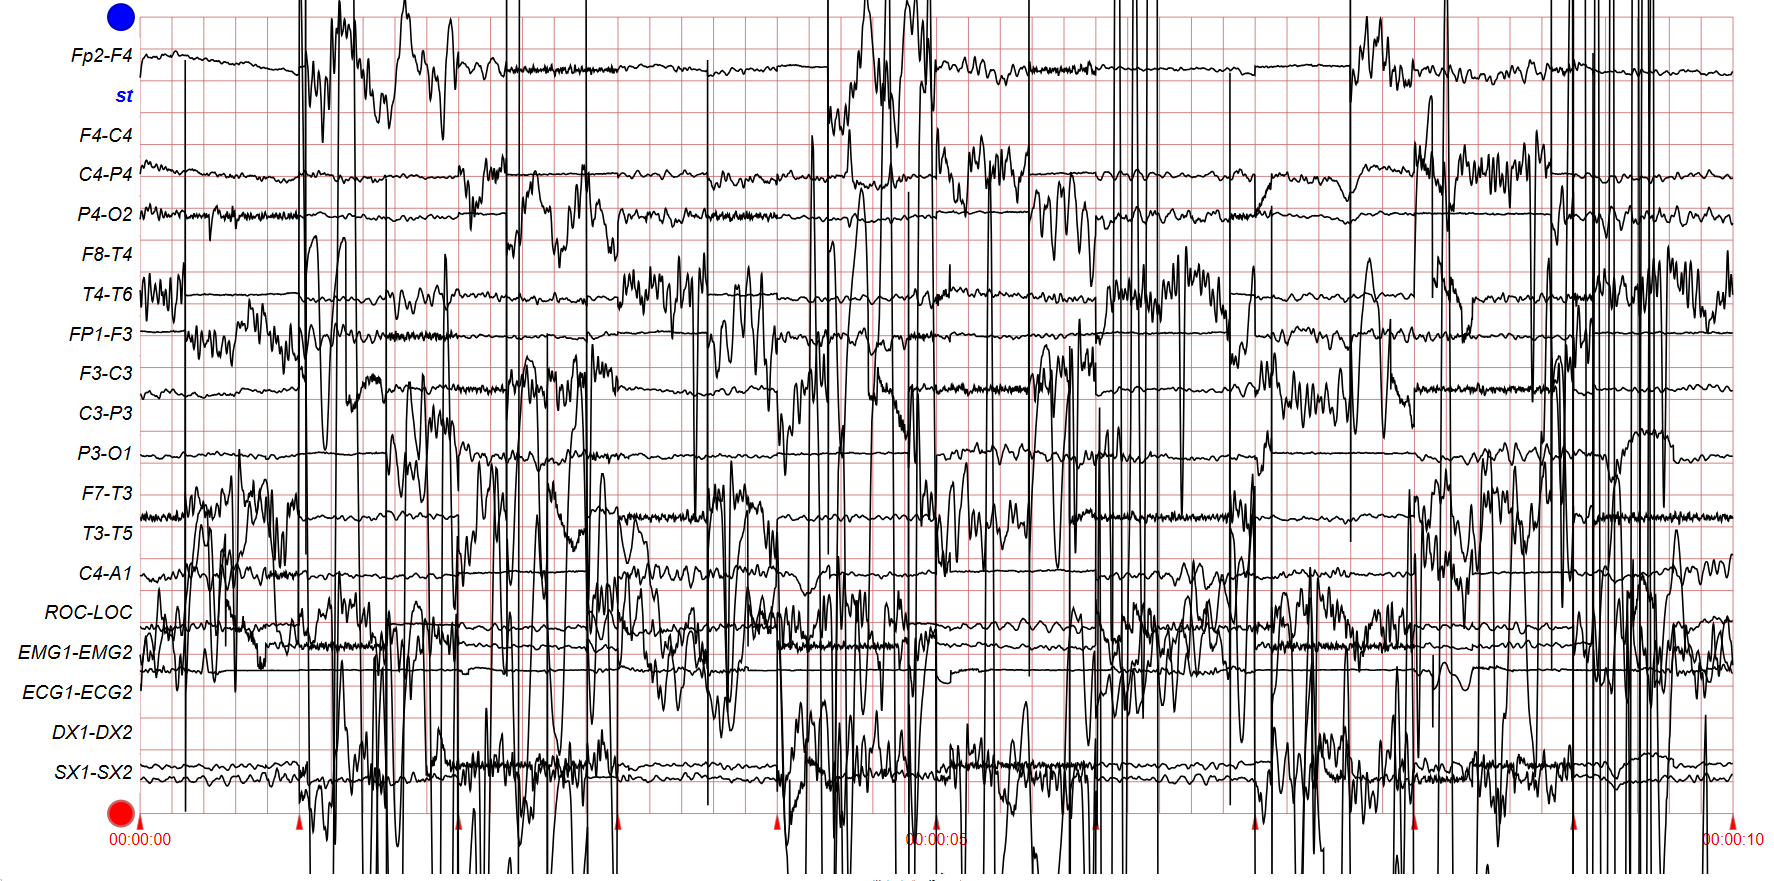
\includegraphics[width=1\linewidth]{Figures/physionet.png}
    \caption{10-second PSG segment from one subject in the CAP Sleep Database}
    \label{fig:physionet}
\end{figure}

The EEG recordings in the dataset were collected at varying sampling frequencies, ranging from 100 Hz to 512 Hz, and vary in duration from approximately 2 to 9 hours. For the purpose of sleep stage classification, the data was segmented into \textbf{epochs} (fixed length time windows of 30 seconds), which serve as the standard unit of analysis in sleep research. \\

Sleep scoring was performed by trained experts following the Rechtschaffen \& Kales (R\&K) guidelines. Each epoch was labeled with a corresponding sleep stage: W for wakefulness, S1–S4 for non-REM (NREM) stages, and R for Rapid Eye Movement (REM) sleep. \\

The dataset includes recordings from both healthy individuals and patients diagnosed with seven different sleep disorders, namely Insomnia, Bruxism, Narcolepsy, Nocturnal Frontal Lobe Epilepsy (NFLE), Periodic Leg Movement (PLM), REM Behavior Disorder (RBD), and Sleep-Disordered Breathing (SDB).  Among the 108 subjects, 16 are completely healthy, while the remaining 92 participants are diagnosed with sleep disorders. 40 have NFLE, 22 experience RBD, 10 have PLM, 9 suffer from insomnia, 5 are diagnosed with narcolepsy, 4 have sleep-disordered breathing, and 2 are affected by bruxism. \\

The participants' ages range from 14 to 82 years, with an average age of approximately 45 years. The dataset consists of 61\% male participants (66 individuals) and 38\% female participants (42 individuals). A summary of these demographic and diagnostic details is presented in Table \ref{tab:cap_sleep}.\\

\begin{table}[H]
    \centering
    \small % Reduce font size to 10pt
    \resizebox{0.6\textwidth}{!}{ % Adjust width
    \begin{tabular}{lccc}
        \toprule
        \textbf{Subject Type} & \textbf{N} & \textbf{M/F} & \textbf{Age (Mean ± SD)} \\
        \midrule
        Healthy    & 16  & 7/9  & 32.19 ± 5.55  \\
        Insomnia   & 9   & 4/5  & 60.89 ± 10.53  \\
        Bruxism    & 2   & 2/0  & 28.5 ± 7.78  \\
        Narcolepsy & 5   & 2/3  & 31.6 ± 11.55  \\
        NFLE       & 40  & 21/19  & 30.28 ± 10.89  \\
        PLM        & 10  & 7/3  & 55.10 ± 6.71  \\
        RBD        & 22  & 19/3  & 70.72 ± 6.37  \\
        SBD        & 4   & 4/0  & 71.25 ± 7.23  \\
        \midrule
        \textbf{Total} & 108  & 66/42 & \textbf{45.19 ± 19.56} \\
        \bottomrule
    \end{tabular}
    }
    \caption{Summary of CAP Sleep Database}
    \label{tab:cap_sleep}
\end{table}


Despite the rich data available in the CAP Sleep Database, most existing studies focus on cyclic phase detection rather than sleep stage classification. While many datasets have been used for sleep stage detection, only few research has specifically utilized the CAP Sleep Database for this purpose.

\section{Data Acquisition for Research}
Subjects  whom had EEG recordings sampled at 512 Hz were selected for this study. 80 subjects, including 6 healthy individuals and 74 individuals with sleep disorders were selected accordingly. Further details for selected subjects on the total number of epochs for each sleep stage across different patient groups are provided in Table \ref{tab:sleep_stages}. Each row in the table corresponds to a specific sleep stage Wake, S1, S2, S3, S4, and REM while each column represents the number of 30 second epochs recorded for that stage across different subject groups. The final two columns summarize the total number of epochs per sleep stage and their corresponding percentage relative to the overall dataset \\

\begin{table}[H]
    \centering
    \resizebox{\textwidth}{!}{ 
    \begin{tabular}{l | r  r r r r r r r | r r} 
        \toprule
        
        Sleep Stage & Healthy & Insomnia & Bruxism & Narcolepsy & NFLE & PLM & RBD & SBD & Total &  (\%) \\
        \midrule
        Wake & 445 & 3801 & 44 & 1303 & 3155 & 1332 & 5266 & 495 & 15841 & 19.64\% \\
        S1   & 280 & 223  & 34  & 301  & 1098 & 266  & 1048  & 269 & 3519  & 4.36\% \\
        S2   & 2172 & 2456 & 144 & 1708 & 10630 & 2748 & 7486 & 1324 & 28628 & 35.50\% \\
        S3   & 573 & 670  & 39  & 476  & 2987  & 955  & 2880  & 224  & 8804  & 10.92\% \\
        S4   & 1184 & 415  & 99  & 568  & 4108  & 956  & 2506  & 352  & 10188 & 12.63\% \\
        REM  & 1409 & 986  & 67  & 1258 & 4905  & 1317 & 3530  & 215  & 13687 & 16.97\% \\
        \midrule
        Total & 6063 & 8551 & 427 & 5614 & 26883 & 7574 & 22676 & 2879 & \textbf{80667} & \textbf{100\%}\\
        \bottomrule
    \end{tabular}
    } % End of resizebox
    \caption{Sleep stage wise details of epoch distribution for selected subjects}
    \label{tab:sleep_stages}
\end{table}


Then created 9 distinct data subsets, namely: Healthy, Insomnia, Bruxism, Narcolepsy, NFLE, PLM, RBD, SDB, and All Subjects Combined. Sleep stage classification was performed separately on each subset. \\

For each data subset, a detailed description of each subset is provided below:

\begin{enumerate}
    \item \textbf{Healthy (DS1):} This subset includes sleep stage epochs from individuals with no reported sleep disorders. It consists of 6 healthy subjects, with a total of 6,063 epochs.
    
    \item \textbf{Insomnia (DS2):} This subset contains sleep stage epochs from 7 individuals diagnosed with insomnia, totaling 8,551 epochs. 
    
    \item \textbf{Bruxism (DS3):} This dataset includes 427 epochs from 1 individual affected by bruxism sleep disorder. 
    
    \item \textbf{Narcolepsy (DS4):} It consists of data from 5 individuals, comprising 5,614 epochs.
    
    \item \textbf{NFLE (DS5):} This subset includes 26,883 epochs from 27 individuals diagnosed with nocturnal frontal lobe epilepsy (NFLE). 
    
    \item \textbf{PLM (Periodic Leg Movement Disorder) (DS6):} It contains 7,574 epochs obtained from 9 individuals with PLM. 

    \item \textbf{RBD (REM Behavior Disorder) (DS7):} This dataset comprises 22,676 epochs collected from 22 individuals diagnosed with RBD. 

    \item \textbf{SDB (Sleep-Disordered Breathing) (DS8):} It includes 2,879 epochs from 3 individuals diagnosed with SDB. 

    \item \textbf{All Subjects Combined (DS9):} This dataset includes data from all 80 subjects, encompassing both healthy and disordered individuals, with a total of 80,667 epochs. 
    
\end{enumerate}

Each PSG recording contained several types signals. We have only used EEG, EOG, ECG and EMG channels for this study.




